\chapter{Introduction}
\label{sec:intro}
\setstretch{\lspac}

\section{The rise of permutation tests}

Provided with the task of investigating an association between two variables from a number of samples, how to quantify the likelihood that a measurement of such association is not merely due to chance? If no true association exists, any pairing of values is incidental, and for a given measurement of one variable, the other could have taken any value. We could thus replace one variable by a set of random values, recompute the association, and keep repeating this procedure multiple times to have a sense of how the association varies when there is no actual effect. \emph{Any} value, as suggested above, however, is not realistic: possible values and their frequencies lie within certain sets or intervals, and occur with frequencies that are not always known. The observed data, however, gives an indication of the possible values and their frequencies. Instead of replacing one variable by sets of random values, the observations for that variable can be \emph{permuted} randomly, the association quantified and recorded, and the process repeated many times. How often a stronger association than the one observed without any permutation, is the answer being sought.

Permutation tests, in their essence, do exactly as above, and despite this simplicity, they entail an obvious practical difficulty: the need to repeat the shuffling many times. Before computers became available, recalculating a measurement of association between variables thousands of times was beyond the bounds of feasibility, rendering them ``little more than curiosities'' \citep{Bradley1968}. The fact that Fisher, their most prominent early proponent \citep{Fisher1935} became silent about these tests in his later years \citep{Basu1980} certainly did not help much to increase their popularity. In practice, only the simplest cases could be performed, although some shortcuts, mostly based on ranks, were eventually developed \citep{Wilcoxon1945, Mann1947, Box1955}. With the possibility of automated execution using computers \citep{Efron1979}, the landscape changed completely, and these otherwise extremely laborious tests became feasible.

Although the idea of repeating an experiment many times while randomising experimental conditions can be traced to the 19th century \citep{Peirce1884}, it was not until the decade of 1930 that strategies started to be studied in depth \citep{Fisher1935, Pitman1937-I, Pitman1937-II, Pitman1938}, notably about the then astonishing idea of shuffling the data that had already been obtained, as opposed to repeating the experiment multiple times. Theoretical and practical advances have been ongoing ever since \citep{Pearson1937, Scheffe1943, Lehmann1949, Kempthorne1955, Freedman1983, Westfall1993, Edgington1995, Good2002, Good2005, Westfall2008, Pesarin2010}; a detailed, extensive historical account is provided by \citet{Berry2014}.

Quite often, permutation tests are presented as an alternative, or in contradistinction, to parametric approaches. This need not be the case: permutation tests do not depend on parametric methods for their existence, and were not created as a direct response or as an alternative to limitations of parametric ones. On the contrary: parametric methods and the assumptions they entail were introduced to solve practical problems at a time in which the ability to perform large number of computations was beyond even the most epic efforts. One could speculate that if computers already existed before the 20th century, parametric methods such as the $t$-test or the $F$-test would have never been devised as known today; perhaps not even inverse probability, from the 17th century and recently in vogue again, would have been developed had computers been available at the time. However, permutation tests did benefit from the parametric literature in that the latter provides test statistics that have some interesting, desirable properties \citep{Hall1991}.

In fairness, some comparisons could still be made. Differently from parametric tests, permutation methods do not depend on underlying theoretical distributions, do not suffer from not quite as stringent assumptions (normality, independence, homogeneous variances), allow the use of non-random samples even of small sizes, and permit a wider variety of test statistics such as those that have poorly known distributions. They are also relatively resilient to outliers (and robust statistics can be used, even without a limiting distribution). All the information necessary for inference is contained in the data itself, not on some idealised population or frequency distribution. An assumption is however needed, the one of exchangeability, that is, that the data after shuffling remain just as likely as the original.

In the brain imaging field, parametric inference using the general linear model \citep[\textsc{glm};][]{Scheffe1959, Searle1971, Friston1994} has, for various reasons, been the stock method: the same framework is treated as applicable to diverse imaging modalities, can be very fast, are well understood, were the first to be available in software packages and, among other benefits, are relatively robust to certain departures from its assumptions. These assumptions refer to (\textsc{i}) having observations that are independent, (\textsc{ii}) that have the same variance, and (\textsc{iii}) that are normally distributed. In one way or another, these can be violated: repeated measurements, subjects that are recruited based on familial relationship with other subjects in the same sample, effects or confounds that affect the variance, lack of normality, non-linear effects, different physical properties and information content of different imaging modalities, among others.

On top of this, there is the multiple testing problem: the parametric solution builds on properties of a random field that must satisfy a myriad of other suppositions: the probability distribution must be the same across space, the field must be a sufficiently ``good'' lattice representation of an underlying continuous process, which on its turn implies that the field must be smooth, and that this smoothness is larger than the voxel size. Plus, the smoothness must be known or estimable at each point, and (ideally) that it is the same for all positions. Moreover, it is also required that the spatial autocorrelation function is twice differentiable at the origin, that the field is thresholded at high levels, and that supra-threshold regions do not touch the borders of the segment of the field that is being inspected. Furthermore, direct results are currently available only for fields that are either Gaussian, or that can be directly related to a Gaussian distribution, as $t$, $F$, $\chi^2$ and $T^2$ \citep{Worsley1996}.

Permutation tests obviate all such issues, that are mostly intrinsic to parametric approaches. In the imaging literature, they were proposed by \citet{blair1994_thatcher} and \citet{Holmes1996}; subsequent, relevant work has been done for various cases and applications \citep{Arndt1996, Locascio1997, Brammer1997, Belmonte2001, Bullmore1996, Bullmore1999, Bullmore2001, Nichols2002, Breakspear2004, Laird2004, Suckling2004, Hayasaka2004, Meriaux2006, Eklund2012, Ge2012, Winkler2014, Winkler2016_npc, McFarquhar2016}. For all its benefits, and now feasible computing, it is of no surprise that interest in this type of test is expected to increase in the upcoming future.

That future is not quite distant. Two recent developments have further propelled the interest on permutation tests. The first is the ongoing reproducibility crisis, that while not specific to brain imaging and affecting essentially all research areas \citep{Baker2016}, relates to it through applications in the fields of psychology and social sciences mainly, but also medical sciences, physics and engineering; it also relates simply for suffering from similar vices and practices \citep{Carp2012, Gorgolewski2016}. While the causes for the crisis are multiple \citep{Eicken2013, Begley2015} and outside the scope of this thesis, there is little doubt that poor statistical practices and too liberal test levels account for some of the ease with which non-existing effects can be labelled as significant \citep{Ioannidis2011}. Studies that lead to p-values too close to the test level, and that rely on too many assumptions are those most vulnerable to errors if such assumptions are not met.

This brings to the second recent development: the finding that at least one of the prevailing parametric strategies used for inference in brain imaging, the one that computes p-values for the size of clusters of voxels that survive a predefined threshold using the aforementioned random field theory, yields unacceptably high false positive rates \citep{Eklund2016}, precisely because some of its suppositions are not met. Permutation tests offer a remedy to issues such as these, provided that their own assumptions, which are fewer and more easily attainable, are satisfied; in some cases, this requires a change of the test statistic.

\section{Overview of the thesis}

Statistics occupy a prominent place in the assessment of brain imaging data. As an example, consider the core analysis tools currently available in the \textsc{fmrib} Software Library (\textsc{fsl}), which are depicted as a flow chart in Figure~\ref{fig:fsl}. Direct statistical modelling and inference are present in the tools \textsc{film}, \textsc{flame}, \texttt{randomise} and \textsc{palm}, with the first two using parametric methods; statistics also play a key role in all other tools. A single statistical framework, if used for various imaging modalities, is more likely to be successful if based on a minimal set of assumptions, for which permutation methods are strong candidates.

\begin{figure}[!b]
\caption[Flow chart of the main analysis methods available in \textsc{fsl}.]{\emph{(page \pageref{fig:fsl_noref})} Flow chart of the main analysis methods available in \textsc{fsl}. Statistical methods occupy a central role, with \textsc{film}, \textsc{flame}, \texttt{randomise}/\textsc{palm}, \textsc{rft} and \textsc{fdr}. In particular, permutation methods occupy a privileged, central position: with the exception of single-subject \textsc{fmri}, all strategies for analysis can pass through \texttt{randomise} or \textsc{palm}.}
\label{fig:fsl}
\end{figure}

\begin{figure}[!p]
\begin{center}
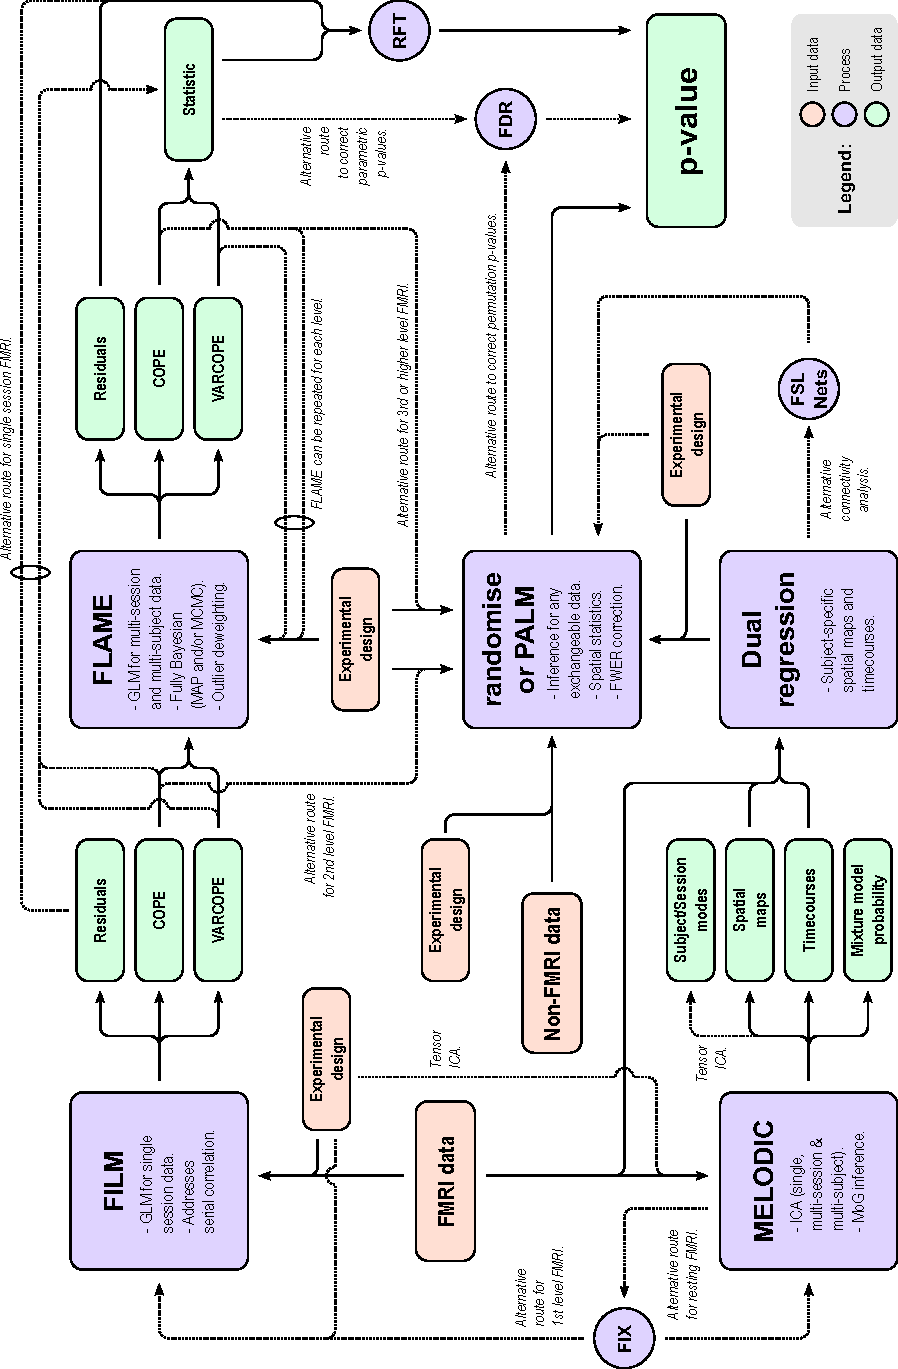
\includegraphics[width=\textwidth]{figures/fsl.pdf}
\end{center}
\label{fig:fsl_noref}
\end{figure}

In the example of \textsc{fsl}, although \texttt{randomise} already covers the most common types of experimental design, currently it does not address various other useful possibilities that include, for instance, (\textsc{i}) statistics that are robust to heteroscedasticity, (\textsc{ii}) multivariate methods, (\textsc{iii}) flexibility to accommodate designs with repeated measurements, (\textsc{iv}) correction for multiple testing based on minimal assumptions, not only across voxels, but also across multiple contrasts and multiple designs, (\textsc{v}) inference with missing data, (\textsc{vi}) multi-level inference on complete generality, for fixed-, random-, and mixed-effects, and (\textsc{vii}) all these performed in a reasonable amount of time even for large datasets. The absence of these techniques is not merely a lack of implementation in \textsc{fsl} or other software: some these topics have only been superficially covered by the literature, with even less work having addressed aspects that are specific to neuroimaging.

In this doctoral thesis, methods for the items (\textsc{iii}) and (\textsc{vii}) are introduced, thus widening the applicability of permutation tests to more cases than otherwise possible; the respective papers have been published \citep{Winkler2015, Winkler2016_fast}. Item (\textsc{i}) was discussed in \citet{Winkler2014}, which is not part of this thesis; likewise items (\textsc{ii}) and (\textsc{iv}) were presented in \citet{Winkler2016_npc}, also not part of this thesis. Items (\textsc{v}) and (\textsc{vi}) are left as future work. This thesis also explores an application of a permutation-based multivariate method, item (\textsc{ii}) above, using the theory presented in \citep{Winkler2016_npc} as the foundation that allows the replacement of analyses of the volume of the cerebral cortex for a joint analysis cortical thickness and cortical surface area. The respective paper is, at the time of this writing, under review, and a pre-print is publicly available in the \emph{bioRxiv} server \citep{Winkler2016_joint}.

Each chapter is a self-contained piece of work, under the common motif that is the extension of possible uses of permutation tests. Each individual chapter can be read together with the others or in isolation, although there is some intertextual elements, particularly on what concerns \textsc{npc}, that appears in Chapters \ref{sec:accel} and \ref{sec:cortex}. All three chapters build on previous research from the author, in particular \citet{Winkler2014, Winkler2016_npc}, but also, to some extent, \citet{Winkler2010, Winkler2012}. However, none of these readings are strictly necessary, and each chapter provides an introduction with a review of the relevant literature.

\subsection{Permutation under structured dependence}

In Chapter~\ref{sec:ptree} we propose a solution to a crucial problem that arises when using permutation tests for the analysis of experimental data using repeated measurements, which, depending on the hypothesis, violates exchangeability: the various measurements obtained from a given subject are not independent from each other, thus not exchangeable. Another case is for data such as those from the Human Connectome Project \citep[\textsc{hcp};][]{VanEssen2012,VanEssen2013}: as each subject does not constitute an independent observation --- many are twins, with additional siblings also participating of the study --- conventional permutation strategies, despite their superior properties in general, if used, would dangerously expose the researcher to an increased risk of false positives.

We address this problem by constructing the permutations in a way that respects the data structure, without the need to explicitly model such structure, by imposing restrictions on exchangeability. Observations are organised in blocks, which are nested within other blocks in a multi-level fashion; these blocks can be shuffled a whole, and inside them, sub-blocks are further allowed to be shuffled, in a recursive process. The method is flexible enough to accommodate permutations, sign-flippings \citep[sometimes also called \emph{wild bootstrap};][]{Guillaume2014}, and permutations together with sign-flippings. In particular, this permutation scheme allows the data such as those from the \textsc{hcp} to be analysed via permutations: subjects are allowed to be shuffled with their siblings while keeping the joint distribution intra-sibship maintained. Then each sibship is allowed to be shuffled with others of the same type, ultimately ensuring that the false positive rate is controlled at the level of the test.

The results from this chapter show that the error type \textsc{i} is controlled at the nominal level, and the power is just marginally smaller than that would be obtained by permuting freely if that were allowed. The more complex the block structure, the larger the reductions in power, although with large sample sizes, the difference reduces. Importantly, simply ignoring family structure in designs as this causes the error rates not to be controlled, with excess false positives, and invalid results. We show examples of false positives that can arise, even after correction for multiple testing, when testing associations between cortical thickness, cortical area, and measures of body size, such as height, weight, and body-mass index, all which are known to be highly heritable. Such false positives can be avoided with permutation tests that respect the family structure.

\subsection{Accelerating permutation tests}

For small sample sizes, low resolutions, or small regions of interest, a permutation test can run very quickly (in a matter of minutes with current personal computers). For larger data, however, they become computationally intensive, and accelerations become useful. The natural strategies to increase the speed consist of the use of faster computers, parallel processing, graphical processing units (\textsc{gpu}s), or use of optimised code. These are general methods that can be considered to various applications.

Instead, Chapter~\ref{sec:accel} does not build on such generic software or hardware improvements, but on properties of certain test statistics and other statistical devices. We evaluate six different strategies for acceleration --- some already existing in the literature, others introduced, improved, or adapted for brain imaging. These strategies allow accelerations larger two orders of magnitude, yielding nearly identical results as in the non-accelerated case. Some, such as tail approximation, are generic enough to be used in nearly all the most common scenarios, including univariate and multivariate tests, spatial statistics, and for correction for multiple testing.

In addition to accelerating the tests, some of these methods considered allow continuous p-values to be obtained, and refine them far into the tail of the distribution of the test statistic, thus avoiding the usual discreteness of p-values in permutation methods, which can be a problem in some applications if too few permutations are done. Based on the results of extensive simulations and on the reanalysis of previously published real data \citep{Douaud2007}, we provide a set of recommendations for cases in which each method should be preferred.

\subsection{Application to cortical morphometry}

A joint, combined analysis of multiple variables can be done using the \emph{non-parametric combination} (\textsc{npc}). While \textsc{npc} is only relatively new \citep{Pesarin2010}, its use in neuroimaging was impossible for two reasons: the need to store very large amounts of data, and low power caused by the fact that, in imaging, correction for multiple testing is mandatory. In a work unrelated to this thesis, \citet{Winkler2016_npc} have made modifications to the original \textsc{npc} so as to render it feasible, valid, and powerful for brain imaging, addressing specific details that include multiple testing and the treatment of spatial statistics.

In Chapter~\ref{sec:cortex}, the application of this modified \textsc{npc} to structural imaging reveals something quite remarkable: that there is a viable way to assess cortical volume that, differently than the wildly popular voxel-based morphometry (\textsc{vbm}), does not mirror the cortical surface area. More: the method is able to reveal patterns of cortical pathology that affect thickness and area in opposing directions --- something that \textsc{vbm} cannot do --- and that even jointly remain a directional test, i.e., not two-tailed, thus in contrast with classical tests such as \textsc{mancova}, which are unable disambiguate directional effects.

Given that thickness and surface area have quite recently been shown to reflect distinct biological processes, cortical volume could still find use for the study of disorders that affect both cortical area and thickness. Here we demonstrate that \textsc{npc} is a better suited solution, that remain superior even when employing an improved, analytic method to measure volume, that is also novel and introduced in this thesis, and that will become the default in the next major release of the FreeSurfer software package.

In the same chapter we also provide, obiter dictum, a comparison of the four existing methods for areal resampling, answering a well known question that had so far not been approached in the literature: can the simple nearest neighbour method for areal interpolation be trusted? The answer is a confident yes, provided that there is smoothing. This translates into substantial gains for those interested, as the alternative, exact method, is computationally too intensive. The chapter equips researchers focused in the in vivo study of cortical anatomy with the information necessary to make the best use of the state-of-the-art morphometry methods.